\newpage
\section{ETL-Definition[EK]}
„ETL (oder Extrahieren, Transformieren, Laden) ist ein Prozess der Datenintegration, welcher drei Schritte umfasst: Extraktion, Transformation und Laden. Kurz gesagt, entnimmt ETL Rohdaten aus mehreren Quellen, konvertiert sie für die Analyse und lädt diese Daten in ihr Warehouse“ \cite{ETL-Explained}
\begin{figure}[H]
    \centering
    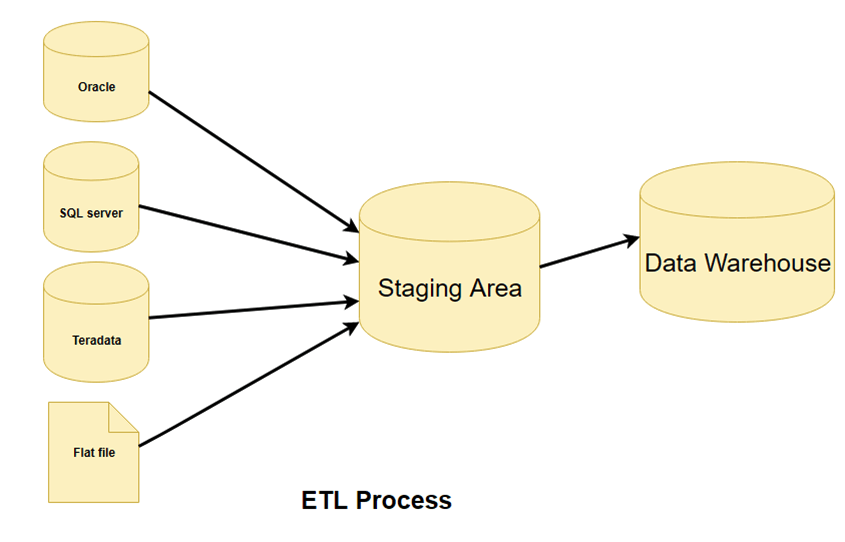
\includegraphics[scale=0.5]{images/etl-staging-area.png}
    \caption{ETL-Staging-Area (02.04.2020)}
    \url{https://www.guru99.com/images/1/022218_0848_ETLExtractT1.png}
\end{figure}
Wie aus der Grafik zu entnehmen ist, kann man den ETL-Prozess neben der Unterteilung in Extraktion, Transformation und Laden auch in diese drei Sektionen unterteilen: Datenquellen, Staging-Area und das Data-Warehouse.


\newpage
\section{Extract[EK]}\label{sec:extract}
Ein jeder ETL-Prozess beginnt mit der Extraktion der zu verarbeitenden Daten. Diese Daten können aus verschiedensten Quellen kommen und eine große Variation in ihrer Strukturierung aufweisen. Somit sollten diese Daten zuerst aufbereitet werden, da ein direkter Transfer ins Data-Warehouse für fehlerhafte und damit unverwendbare Daten sorgen könnte. Verschiedenste Gründe können dafür vorliegen. Es können die Daten von der Quelle selbst bereits beschädigt sein, oder durch ihre Vielzahl an Datenformaten zu einer Unvereinbarkeit dieser kommen.
\vspace{5mm}\par
Um hier Abhilfe zu schaffen, kommen die Daten zuerst in eine sogenannte Staging-Area. Diese wird dafür verwendet, um die Daten so aufzubereiten, dass in ihnen nur noch die Informationen enthalten sind, welche vom Data-Warehouse benötigt werden und in solch einer Form, dass diese vereinheitlicht organisiert sind. Darüber hinaus entsteht ein Möglichkeitsfenster, um diese Daten auch zu validieren, was je nach Datenquelle mehr oder weniger von Nöten ist. Folgend ein paar Beispiele, welche aufzeigen sollen, welche Möglichkeiten der Validierung während der Extraktion vorliegen:
\begin{itemize}
  \item Abgleichen von Datensätzen mit der Quelle
  \item Überprüfung der Richtigkeit der Datentypen
  \item Entfernen von Duplikaten
  \item Entfernen von fragmentierten Daten
\end{itemize}
Ein wichtiger Punkt des Extrakts ist, dass die Abfrage der Daten aus der Quelle für keine Performanceeinbußen sorgen sollte. Die Begründung dafür ergibt sich aus einer Tatsache. Meist kommen die Daten, welche für einen ETL-Prozess von Interesse sind von einem Live-Production-System beziehungsweise einer Datenbank. Das bedeutet, dass es sich bei diesen um systemkritische Elemente handelt, ein Performanceeinbruch könnte schwerwiegende Probleme in der Haupttätigkeit des Systems hervorrufen und bei Unternehmen gar zu Einkommenseinbußen führen. Die Eigenschaften einer guten Extraktion bestehen also darin, dass wir Fehlerquellen vorzeitig abfangen können und dass Daten so direkt wie möglich aus der Quelle entnommen werden - Transformationen sollen, wenn von Nöten erst in der Staging-Area im ETL stattfinden und nicht bei der Abfrage.
(vgl. \cite{ETL-Process} \& \cite{ETL-Explained})